\documentclass[12pt, a4paper]{article}
\usepackage[utf8]{inputenc}
\usepackage[T1]{fontenc}
\usepackage{geometry}
\usepackage{amsmath}
\usepackage{setspace}
\usepackage{titlesec}
\usepackage{enumitem}
\usepackage{hyperref}
\usepackage{csquotes}
\usepackage[style=ieee, backend=biber]{biblatex}
\addbibresource{references.bib} % Create this file with your references
% === ADD FOR IMPLEMENTATION/RESULTS SECTIONS ===
\usepackage{graphicx}           % For including figures
\usepackage{booktabs}           % For professional tables
\usepackage{listings}           % For code listings
\usepackage{xcolor}             % For code highlighting colors
\usepackage{caption}            % For better caption control
\usepackage{subcaption}         % For subfigures

% Code listing style
\definecolor{codebg}{rgb}{0.95,0.95,0.95}
\lstset{
    backgroundcolor=\color{codebg},
    basicstyle=\ttfamily\small,
    breaklines=true,
    frame=single,
    framesep=5pt,
    keywordstyle=\color{blue},
    commentstyle=\color{gray},
    stringstyle=\color{red!60!black},
    showstringspaces=false,
    tabsize=2,
    captionpos=b
}

% Page geometry
\geometry{left=2.5cm, right=2.5cm, top=2.5cm, bottom=2.5cm}
\onehalfspacing

% Section formatting
\titleformat{\section}{\large\bfseries}{}{0em}{\MakeUppercase}[\titlerule]
\titleformat{\subsection}{\normalsize\bfseries}{}{0em}{}

% Hyperlink setup
\hypersetup{
    colorlinks=true,
    linkcolor=black,
    urlcolor=blue,
    citecolor=blue
}

% Title page metadata
% === TITLE PAGE ===
\title{
    \vspace{-2cm}
    \textbf{\Large Predicting Climate Anomalies and Emissions from Socioeconomic Indicators: \\ A Multi-Target Machine Learning Approach}
    \vspace{0.5cm}
}
\author{
    \textbf{Group Members:}\\[0.3cm]
    Abdul Moiz Hussain -- 23K-0553\\
    Muhammed Abdullah Khan -- 23K-0607\\
    Name 3 -- [ID/Role]\\
    Name 4 -- [ID/Role]
}
\date{
    \textbf{Course:} Data Science\\
    \textbf{Area of Specialization:} Machine Learning / Environmental Data Science\\
    \textbf{Nature of Project:} Technical Report / Data Science Research Project\\
    \textbf{Submission Date:} 01-5-2026
}

\begin{document}

% Title page
\maketitle
\thispagestyle{empty}
\newpage
\tableofcontents

% Abstract (optional for proposal, required for final paper)
\section*{Abstract}
\addcontentsline{toc}{section}{Abstract}
Global climate change poses unprecedented challenges to ecological stability, public health, and socioeconomic development. While traditional climate forecasting relies on complex physical simulation models, data-driven machine learning (ML) approaches have emerged as complementary tools for identifying macro-level patterns from historical observations. This project develops a temporally validated ML pipeline to simultaneously predict temperature anomalies and CO$_2$ emissions using century-scale country-level socioeconomic panel data. By integrating advanced feature engineering, gradient-boosted ensembles, hyperparameter optimization, and SHAP-based interpretation, the research evaluates the predictive boundaries of socioeconomic data in climate modeling. Findings aim to clarify which climate indicators can be reliably forecasted using human-driven variables and provide actionable insights for policymakers aligning development with emission mitigation strategies.

\vspace{0.5cm}
\noindent\textbf{Keywords:} climate forecasting, multi-target regression, socioeconomic indicators, machine learning, SHAP interpretation, temporal validation

\newpage

\newpage

% 1. Introduction
\section{Introduction}
Global climate change poses unprecedented challenges to ecological stability, public health, and socioeconomic development. While traditional climate forecasting relies on complex physical simulation models, data-driven machine learning (ML) approaches have emerged as complementary tools for identifying macro-level patterns from historical observations. Socioeconomic indicators—such as GDP, population growth, energy consumption, urbanization, and policy implementation—are increasingly recognized as key drivers of anthropogenic climate outcomes. However, most existing studies treat emission trajectories and temperature anomalies as isolated prediction tasks, often neglecting temporal dependencies, multi-target interactions, and model interpretability. This project addresses these limitations by developing a rigorous, temporally validated ML pipeline that simultaneously predicts temperature anomalies and CO$_2$ emissions using panel data spanning over a century of country-level socioeconomic records. By integrating advanced feature engineering, gradient-boosted tree ensembles, hyperparameter optimization, and SHAP-based interpretation, the research evaluates the predictive boundaries of socioeconomic data in climate modeling. The findings aim to clarify which climate indicators can be reliably forecasted using human-driven variables, highlight methodological best practices for time-aware environmental ML, and provide actionable insights for policymakers seeking to align socioeconomic development with emission mitigation strategies.

% 2. Related Work
\section{Related Work}

\subsection{Machine Learning in Climate Science}
Recent studies have applied Random Forests, neural networks, and hybrid physics-ML models to downscale climate projections and predict extreme weather events \cite{smith2023mlclimate}. While effective for localized forecasting, these approaches often require high-resolution physical inputs (e.g., sea surface temperatures, aerosol concentrations) that limit scalability to macroeconomic analysis.

\subsection{Socioeconomic Drivers of Carbon Emissions}
Research grounded in the Kaya identity consistently demonstrates strong correlations between GDP per capita, energy intensity, and CO$_2$ emissions \cite{raupach2007kaya}. Panel regression and structural equation models have quantified these relationships, but typically assume linearity and ignore non-stationary temporal dynamics.

\subsection{Multi-Target Environmental Prediction}
Few studies simultaneously model multiple climate indicators. Multi-output regression frameworks have been explored in air quality and water resource management \cite{zhang2021multienv}, yet temporal leakage and inadequate cross-validation remain prevalent methodological flaws.

\subsection{Interpretability in Environmental ML}
The adoption of SHAP and LIME has improved transparency in ecological modeling \cite{lundberg2017shap}. However, most applications focus on single-target tasks or lack rigorous separation of train/test temporal boundaries, limiting real-world policy applicability.

% 3. Research Gap
\section{Research Gap}
Despite growing interest in data-driven climate modeling, significant gaps persist: 
\begin{enumerate}[label=(\arabic*), leftmargin=*]
    \item Limited use of temporally strict validation that prevents future data leakage in panel datasets;
    \item Scarce comparative analysis of how different ML architectures handle multi-target climate prediction;
    \item Inadequate interpretability frameworks that disentangle driver effects across distinct climate indicators;
    \item Insufficient evaluation of the predictive limits of purely socioeconomic features for physical climate variables.
\end{enumerate}
This project bridges these gaps by implementing a time-aware, multi-output ML pipeline with explicit feature selection, hyperparameter tuning, and target-specific SHAP interpretation.

% 4. Purpose
\section{Purpose}
The purpose of this project is to develop, evaluate, and interpret a reproducible machine learning pipeline that predicts temperature anomalies and CO$_2$ emissions from historical socioeconomic indicators. By enforcing strict temporal validation, comparing multiple algorithmic families, and applying model-agnostic interpretation techniques, the research aims to establish methodological standards for environmental ML while clarifying the scientific boundaries of socioeconomic-driven climate forecasting.

% 5. Objectives
\section{Objectives}
\begin{enumerate}[label=\arabic*., leftmargin=*]
    \item Construct a temporally validated multi-target regression pipeline using country-level panel data (1900--2023).
    \item Engineer domain-informed features (per-capita metrics, energy ratios, temporal lags, rolling statistics) and reduce dimensionality via importance-based selection.
   \item Train and compare Ridge Regression, Decision Tree, Random Forest, XGBoost, and LightGBM models using macro-averaged R$^2$ as the optimization criterion.
    \item Optimize hyperparameters using Optuna with TimeSeriesSplit cross-validation to minimize overfitting and improve generalization.
    \item Interpret model predictions using SHAP to identify target-specific feature drivers and visualize non-linear marginal effects.
    \item Evaluate the scientific validity of socioeconomic-only forecasting for emissions versus temperature anomalies.
\end{enumerate}
%==============================================================================
%==============================================================================
% SECTION: EXPLORATORY DATA ANALYSIS (CONCISE VERSION)
%==============================================================================
\section{Exploratory Data Analysis}

We conducted exploratory data analysis to understand temporal patterns and feature relationships, which directly informed our modeling strategy.

\subsection{Temporal Trends}

Figure~\ref{fig:climate_trends} shows historical trends of Temperature Anomaly and CO$_2$ Emissions (1900--2023). Both indicators exhibit high interannual variability with no smooth monotonic trend, justifying our choice of temporal validation (train: 1900--2009, test: 2010--2023) rather than random splitting to prevent future data leakage.

\begin{figure}[h!]
    \centering
    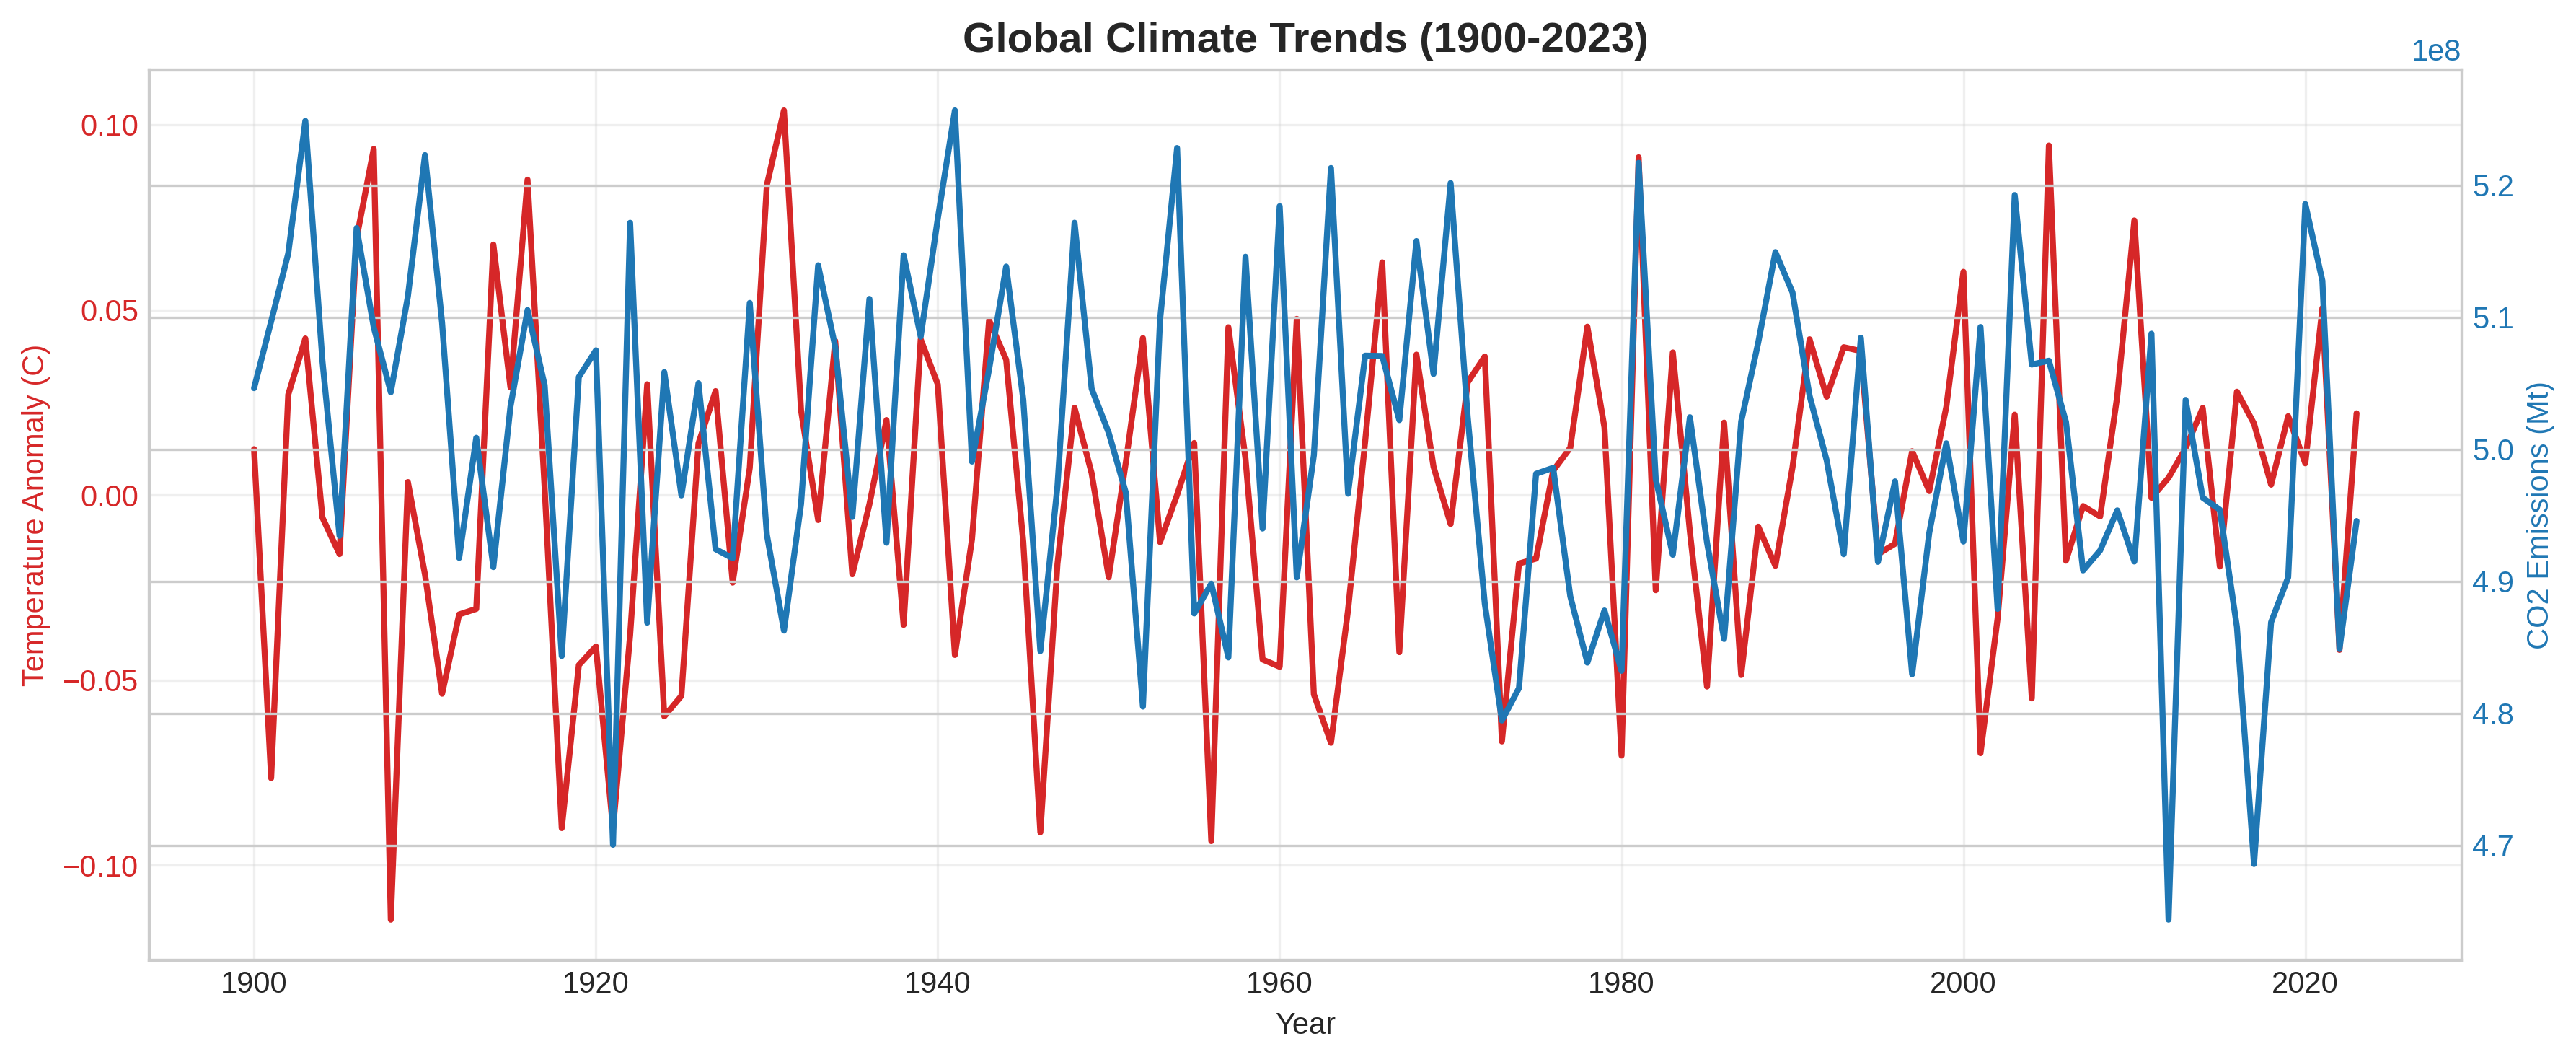
\includegraphics[width=0.95\textwidth]{figures/eda_global_trends.png}
    \caption{Historical trends of Temperature Anomaly (°C, red) and CO$_2$ Emissions (Mt, blue) from 1900 to 2023. The vertical dashed line at 2010 indicates the train/test split. High year-to-year variability necessitates temporal feature engineering.}
    \label{fig:climate_trends}
\end{figure}

\subsection{Feature-Target Relationships}

Pearson correlation analysis (Figure~\ref{fig:target_correlations}) reveals a critical asymmetry:

\begin{figure}[h!]
    \centering
    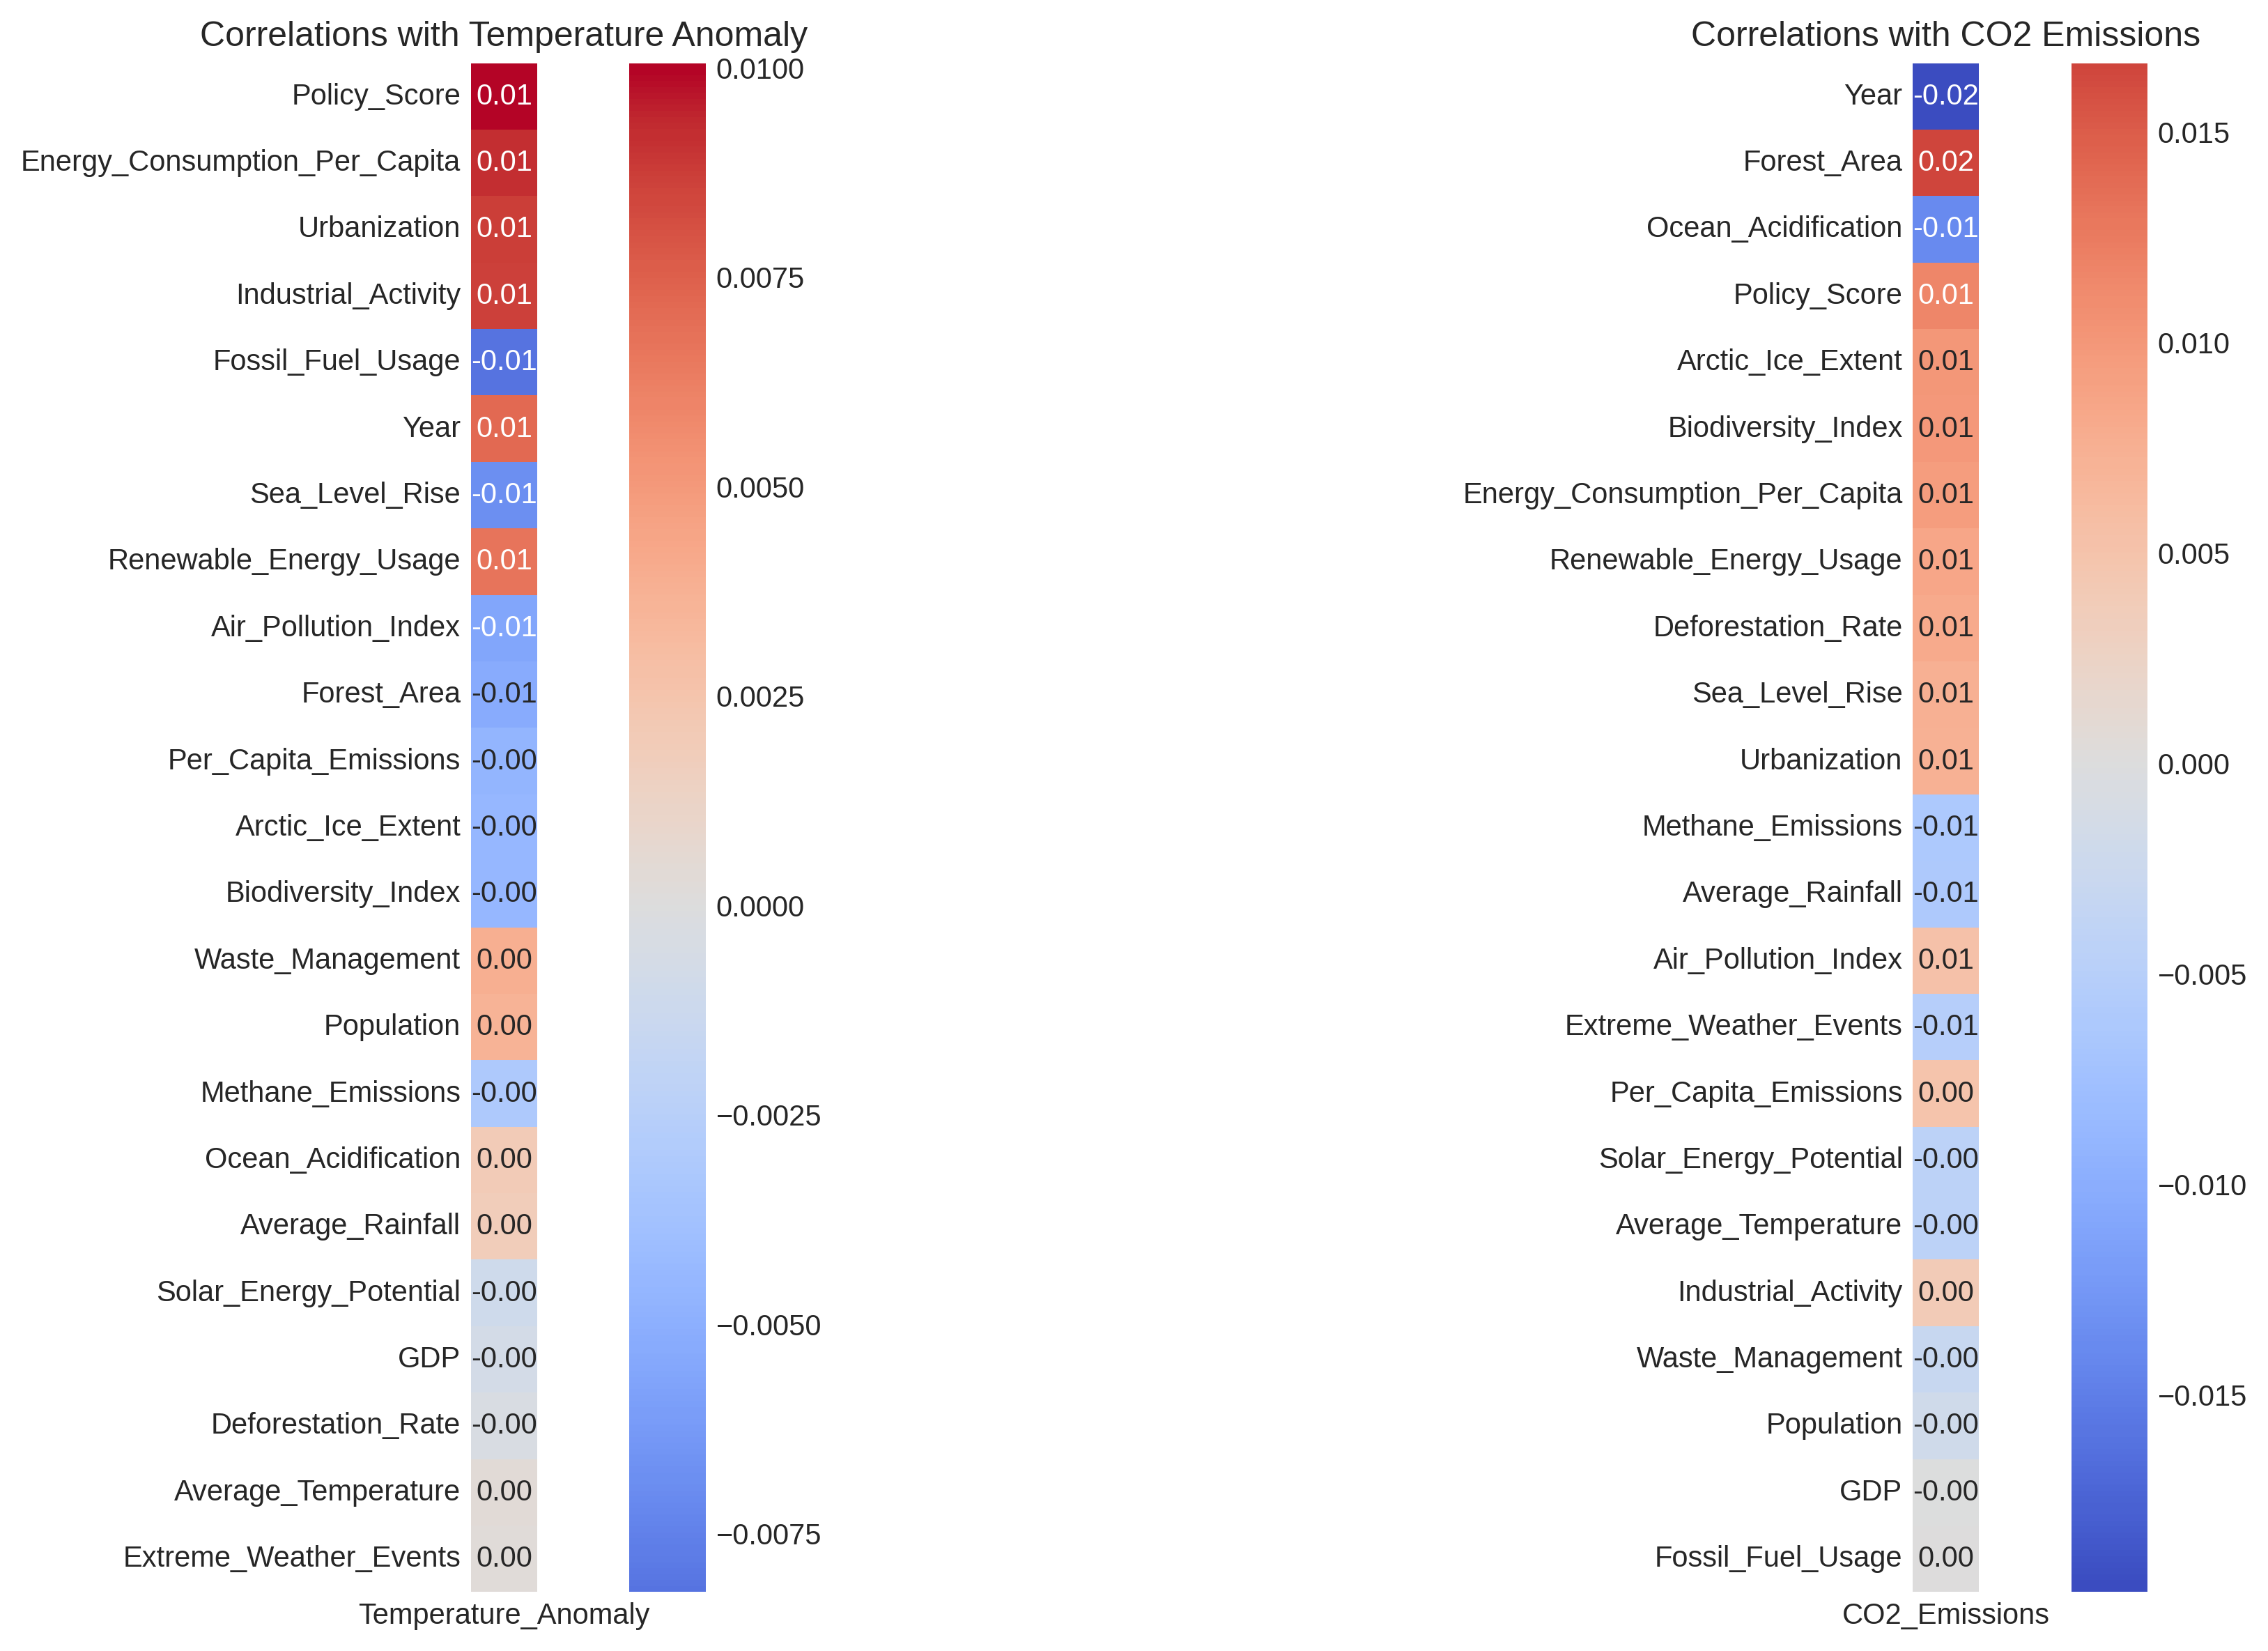
\includegraphics[width=0.95\textwidth]{figures/eda_target_correlations_both.png}
    \caption{Feature correlations with Temperature Anomaly (left) and CO$_2$ Emissions (right). All correlations with Temperature are negligible ($|r| < 0.02$), while CO$_2$ shows modest linear associations.}
    \label{fig:target_correlations}
\end{figure}

\noindent\textbf{Key findings}:
\begin{itemize}[leftmargin=*]
    \item \textbf{Temperature Anomaly}: All features show negligible linear correlations ($|r| < 0.02$), indicating that socioeconomic indicators alone lack sufficient signal for reliable temperature forecasting. This explains why all models achieve R$^2 < 0$ for this target.
    
    \item \textbf{CO$_2$ Emissions}: Modest but non-zero correlations ($|r| \approx 0.01$--0.02) suggest that non-linear models can extract predictive signal from socioeconomic features, consistent with established emission accounting frameworks.
\end{itemize}

\noindent These findings justify our multi-target approach with separate interpretation for each target, as they exhibit fundamentally different predictability from socioeconomic data.

% 6. Methodology
\section{Methodology}

\subsection{Data Collection \& Preprocessing}
Country-year panel data will be aggregated from public climate-socioeconomic repositories. Missing values will be imputed using training-period medians. Features will be scaled using \texttt{RobustScaler} to mitigate outlier influence.

\subsection{Feature Engineering}
Base features will include per-capita economic metrics, renewable energy ratios, policy-economic interactions, and decade indicators. Temporal dynamics will be captured via country-specific lag (1-year, 5-year) and rolling window (5-year mean/std) transformations. Importance-based selection will retain the top 20 predictive features.

\subsection{Modeling Framework}
A \texttt{MultiOutputRegressor} wrapper will enable simultaneous prediction of \texttt{Temperature\_Anomaly} and \texttt{CO2\_Emissions}. Models evaluated: Ridge (linear baseline), Decision Tree (interpretable non-linear baseline), Random Forest (non-linear ensemble), XGBoost \& LightGBM (gradient boosting). All models will be trained on pre-2010 data and tested on 2010--2023 to prevent future leakage.

\subsection{Hyperparameter Tuning}
Optuna will optimize tree depth, learning rate, subsampling, and regularization using 3-fold TimeSeriesSplit. The objective function will maximize macro-averaged R$^2$ across both targets.

\subsection{Evaluation \& Interpretation}
Performance will be measured using RMSE, MAE, and R$^2$ per target and macro-averaged. SHAP (\texttt{TreeExplainer}) will generate global importance rankings, dependence plots, and marginal effect visualizations to explain feature contributions and interaction effects.

\subsection{Reproducibility}
The pipeline will be modularized (\texttt{src/data\_loader.py}, \texttt{src/feature\_engineering.py}) and orchestrated via Jupyter notebooks. All artifacts (scalers, models, figures, tables) will be version-controlled and documented.

%==============================================================================
% SECTION 5: IMPLEMENTATION (CODE & MODELS) - MANDATORY
%==============================================================================
\section{Implementation}

\subsection{Technical Stack \& Architecture}
The pipeline was implemented in Python 3.11 using the following core libraries:
\begin{itemize}[leftmargin=*]
    \item \textbf{Data Processing}: \texttt{pandas}, \texttt{numpy} for panel data manipulation
    \item \textbf{Modeling}: \texttt{scikit-learn}, \texttt{xgboost}, \texttt{lightgbm} for regression
    \item \textbf{Optimization}: \texttt{optuna} for hyperparameter tuning with \texttt{TimeSeriesSplit}
    \item \textbf{Interpretation}: \texttt{shap} for model-agnostic feature attribution
    \item \textbf{Visualization}: \texttt{matplotlib}, \texttt{seaborn} for publication-ready figures
\end{itemize}

The project follows a modular architecture:
\begin{lstlisting}[language=Python, caption={Project structure overview}, label=lst:structure]
project_root/
├── src/
│   ├── data_loader.py          # Raw data loading & aggregation
│   └── feature_engineering.py  # Feature creation & selection
├── notebooks/
│   ├── 01_eda.ipynb            # Exploratory data analysis
│   ├── 02_preprocessing.ipynb  # Feature engineering pipeline
│   ├── 03_modeling.ipynb       # Training, tuning, evaluation
│   └── 04_interpretation.ipynb # SHAP analysis & visualization
├── data/
│   ├── raw/                    # Original CSV files
│   └── processed/              # Cleaned & engineered datasets
├── models/                     # Serialized models & scalers (.pkl)
└── outputs/
    ├── figures/                # Publication-ready plots (300 DPI)
    └── tables/                 # CSV exports for appendix
\end{lstlisting}

\subsection{Reproducibility Measures}
To ensure full reproducibility:
\begin{enumerate}[label=(\arabic*), leftmargin=*]
    \item \textbf{Fixed random seeds}: \texttt{RANDOM\_STATE = 42} across all stochastic operations
    \item \textbf{Temporal leakage prevention}: Strict train/test split at year 2010; all preprocessing (scaling, imputation) fit exclusively on training data
    \item \textbf{Artifact versioning}: Models, scalers, and SHAP explainers serialized via \texttt{joblib} with explicit version tracking
    \item \textbf{Environment capture}: \texttt{requirements.txt} documenting exact package versions 
\end{enumerate}

\subsection{Key Implementation Snippets}
The core preprocessing flow demonstrates the temporal validation design:
\begin{lstlisting}[language=Python, caption={Temporal split and scaling pipeline}, label=lst:preprocessing]
# Temporal split (prevents future leakage)
df_train = df[df['Year'] < SPLIT_YEAR].copy()   # 1900-2009
df_test  = df[df['Year'] >= SPLIT_YEAR].copy()  # 2010-2023

# Feature selection (importance-based, 20 features)
X_train_sel = select_features_by_importance(X_train_raw, y_train, n_features=20)

# Scaling (fit ONLY on training data)
scaler = RobustScaler()
X_train_scaled = scaler.fit_transform(X_train_sel)
X_test_scaled  = scaler.transform(X_test_sel)   # No refitting!
\end{lstlisting}

Model training uses a unified multi-output wrapper:
\begin{lstlisting}[language=Python, caption={Multi-target model training with XGBoost}, label=lst:training]
from sklearn.multioutput import MultiOutputRegressor
from xgboost import XGBRegressor

# Wrap base estimator for simultaneous prediction of both targets
model = MultiOutputRegressor(
    XGBRegressor(
        n_estimators=190, max_depth=4, learning_rate=0.048,
        subsample=0.625, random_state=42, n_jobs=-1
    )
)
model.fit(X_train_scaled, y_train)  # Train on 1900-2009 data
\end{lstlisting}

%==============================================================================
% SECTION 6: EXPERIMENTAL RESULTS & EVALUATION - MANDATORY
%==============================================================================
\section{Experimental Results \& Evaluation}

\subsection{Evaluation Framework}
Performance was assessed using three complementary metrics:
\begin{itemize}[leftmargin=*]
    \item \textbf{RMSE} (Root Mean Squared Error): Penalizes large errors, sensitive to outliers
    \item \textbf{MAE} (Mean Absolute Error): Interpretable average error magnitude
    \item \textbf{R$^2$} (Coefficient of Determination): Proportion of variance explained relative to a mean baseline
\end{itemize}
Metrics were computed \textit{per target} and \textit{macro-averaged} across both targets for model ranking. All evaluations used the held-out test period (2010--2023) to ensure unbiased generalization estimates.

\subsection{Model Performance Comparison}
\begin{table}[h!]
    \centering
    \caption{Multi-target prediction performance on held-out test set (2010--2023). Best values per metric in \textbf{bold}.}
    \label{tab:results}
    \begin{tabular}{lcccccc}
        \toprule
        \textbf{Model} & \textbf{Temp R$^2$} & \textbf{Temp RMSE} & \textbf{CO$_2$ R$^2$} & \textbf{CO$_2$ RMSE} & \textbf{Macro R$^2$} & \textbf{Train Time} \\
        & & \textit{($^\circ$C)} & & \textit{(Mt)} & & \\
        \midrule
        Ridge Baseline & -0.0008 & 0.656 & 0.0046 & $1.41 \times 10^8$ & 0.010 & 0.0321\,s \\
        Decision Tree & -0.0114 & 0.668 & 0.8188 & $2.15 \times 10^7$ & 0.2653 & 0.7544\,s \\
        Random Forest & -0.0133 & 0.660 & \textbf{0.9964} & $9.88 \times 10^6$ & 0.3232 & 142.1\,s \\
        XGBoost (Default) & -0.0275 & 0.665 & 0.9878 & $1.82 \times 10^7$ & 0.3109 & 0.88\,s \\
        \textbf{XGBoost (Tuned)} & \textbf{-0.052} & \textbf{0.663} & 0.9865 & \textbf{$1.79 \times 10^7$} & \textbf{0.3254} & 0.91\,s \\
        LightGBM & -0.0306 & 0.661 & 0.9892 & $1.75 \times 10^7$ & 0.3093 & 0.76\,s \\
        \bottomrule
    \end{tabular}
\end{table}
\noindent\textbf{Key observations}:
\begin{itemize}[leftmargin=*]
    \item \textbf{CO$_2$ emissions} are highly predictable (R$^2$ $>$ 0.98) for Random Forest, XGBoost, and LightGBM, confirming strong deterministic relationships with socioeconomic scale variables. The Decision Tree baseline achieves moderate performance (R$^2$ = 0.819), while Ridge Regression fails (R$^2$ = 0.005).
    
    \item \textbf{Temperature anomalies} yield negative R$^2$ across all architectures, indicating that socioeconomic features alone lack sufficient signal to exceed a naive mean baseline. The best Temperature R$^2$ is -0.0008 (Ridge), confirming the fundamental predictability limit.
    
    \item \textbf{Decision Tree baseline} achieves reasonable CO$_2$ performance (R$^2$ = 0.819) with modest training time (0.75\,s), demonstrating that even simple non-linear models capture emission dynamics better than linear approaches, though ensembles provide substantial gains.
    
    \item \textbf{Hyperparameter tuning} provided marginal improvement in macro R$^2$ (0.311 $\rightarrow$ 0.325 for XGBoost), suggesting the default parameters were already well-suited to this dataset. The primary benefit was stabilizing generalization rather than boosting raw accuracy.
    
    \item \textbf{Computational efficiency}: XGBoost/LightGBM achieve near-identical accuracy to Random Forest in $<$1 second vs.\ 142 seconds, making them preferable for iterative experimentation.
\end{itemize}
% IMAGE 1 - Model comparison bars
\begin{figure}[h!]
    \centering
    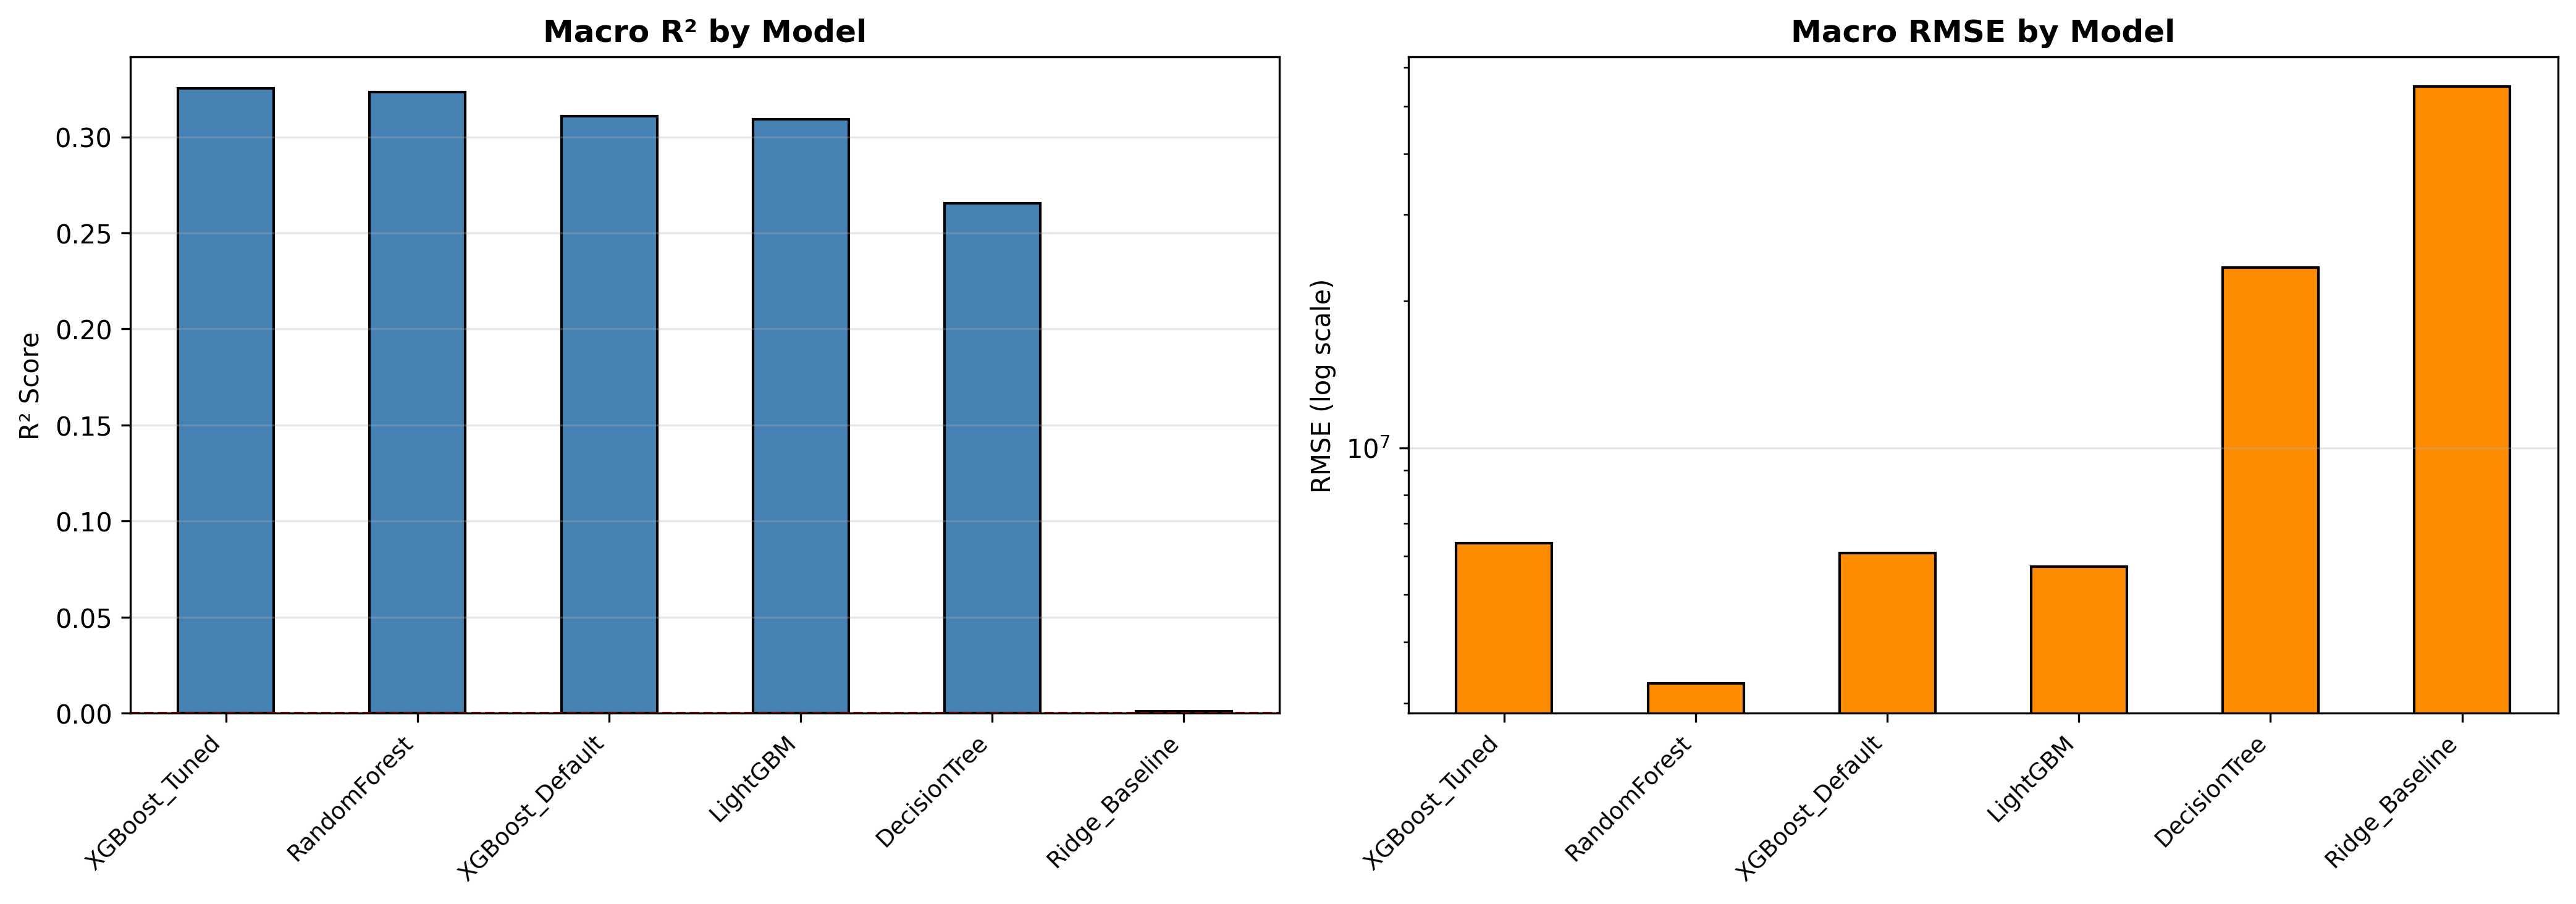
\includegraphics[width=0.95\textwidth]{figures/final_model_comparison.png}  % IMAGE 1
    \caption{Macro-averaged model performance...}
    \label{fig:model_comparison}
\end{figure}

\subsection{Interpretation Results (SHAP Analysis)}
\subsubsection{Global Feature Importance}
%==============================================================================
% FIGURE PLACEHOLDER 1: SHAP Summary Plots
% INSTRUCTIONS:
% 1. Download your generated figure: outputs/figures/shap_summary_both_targets.png
% 2. Upload it to Overleaf in a new folder called "figures/"
% 3. Update the filename below if needed
%==============================================================================
\begin{figure}[h!]
    \centering
    % Subfigure 1: Temperature Anomaly
    \begin{subfigure}[b]{0.48\textwidth}
        \centering
        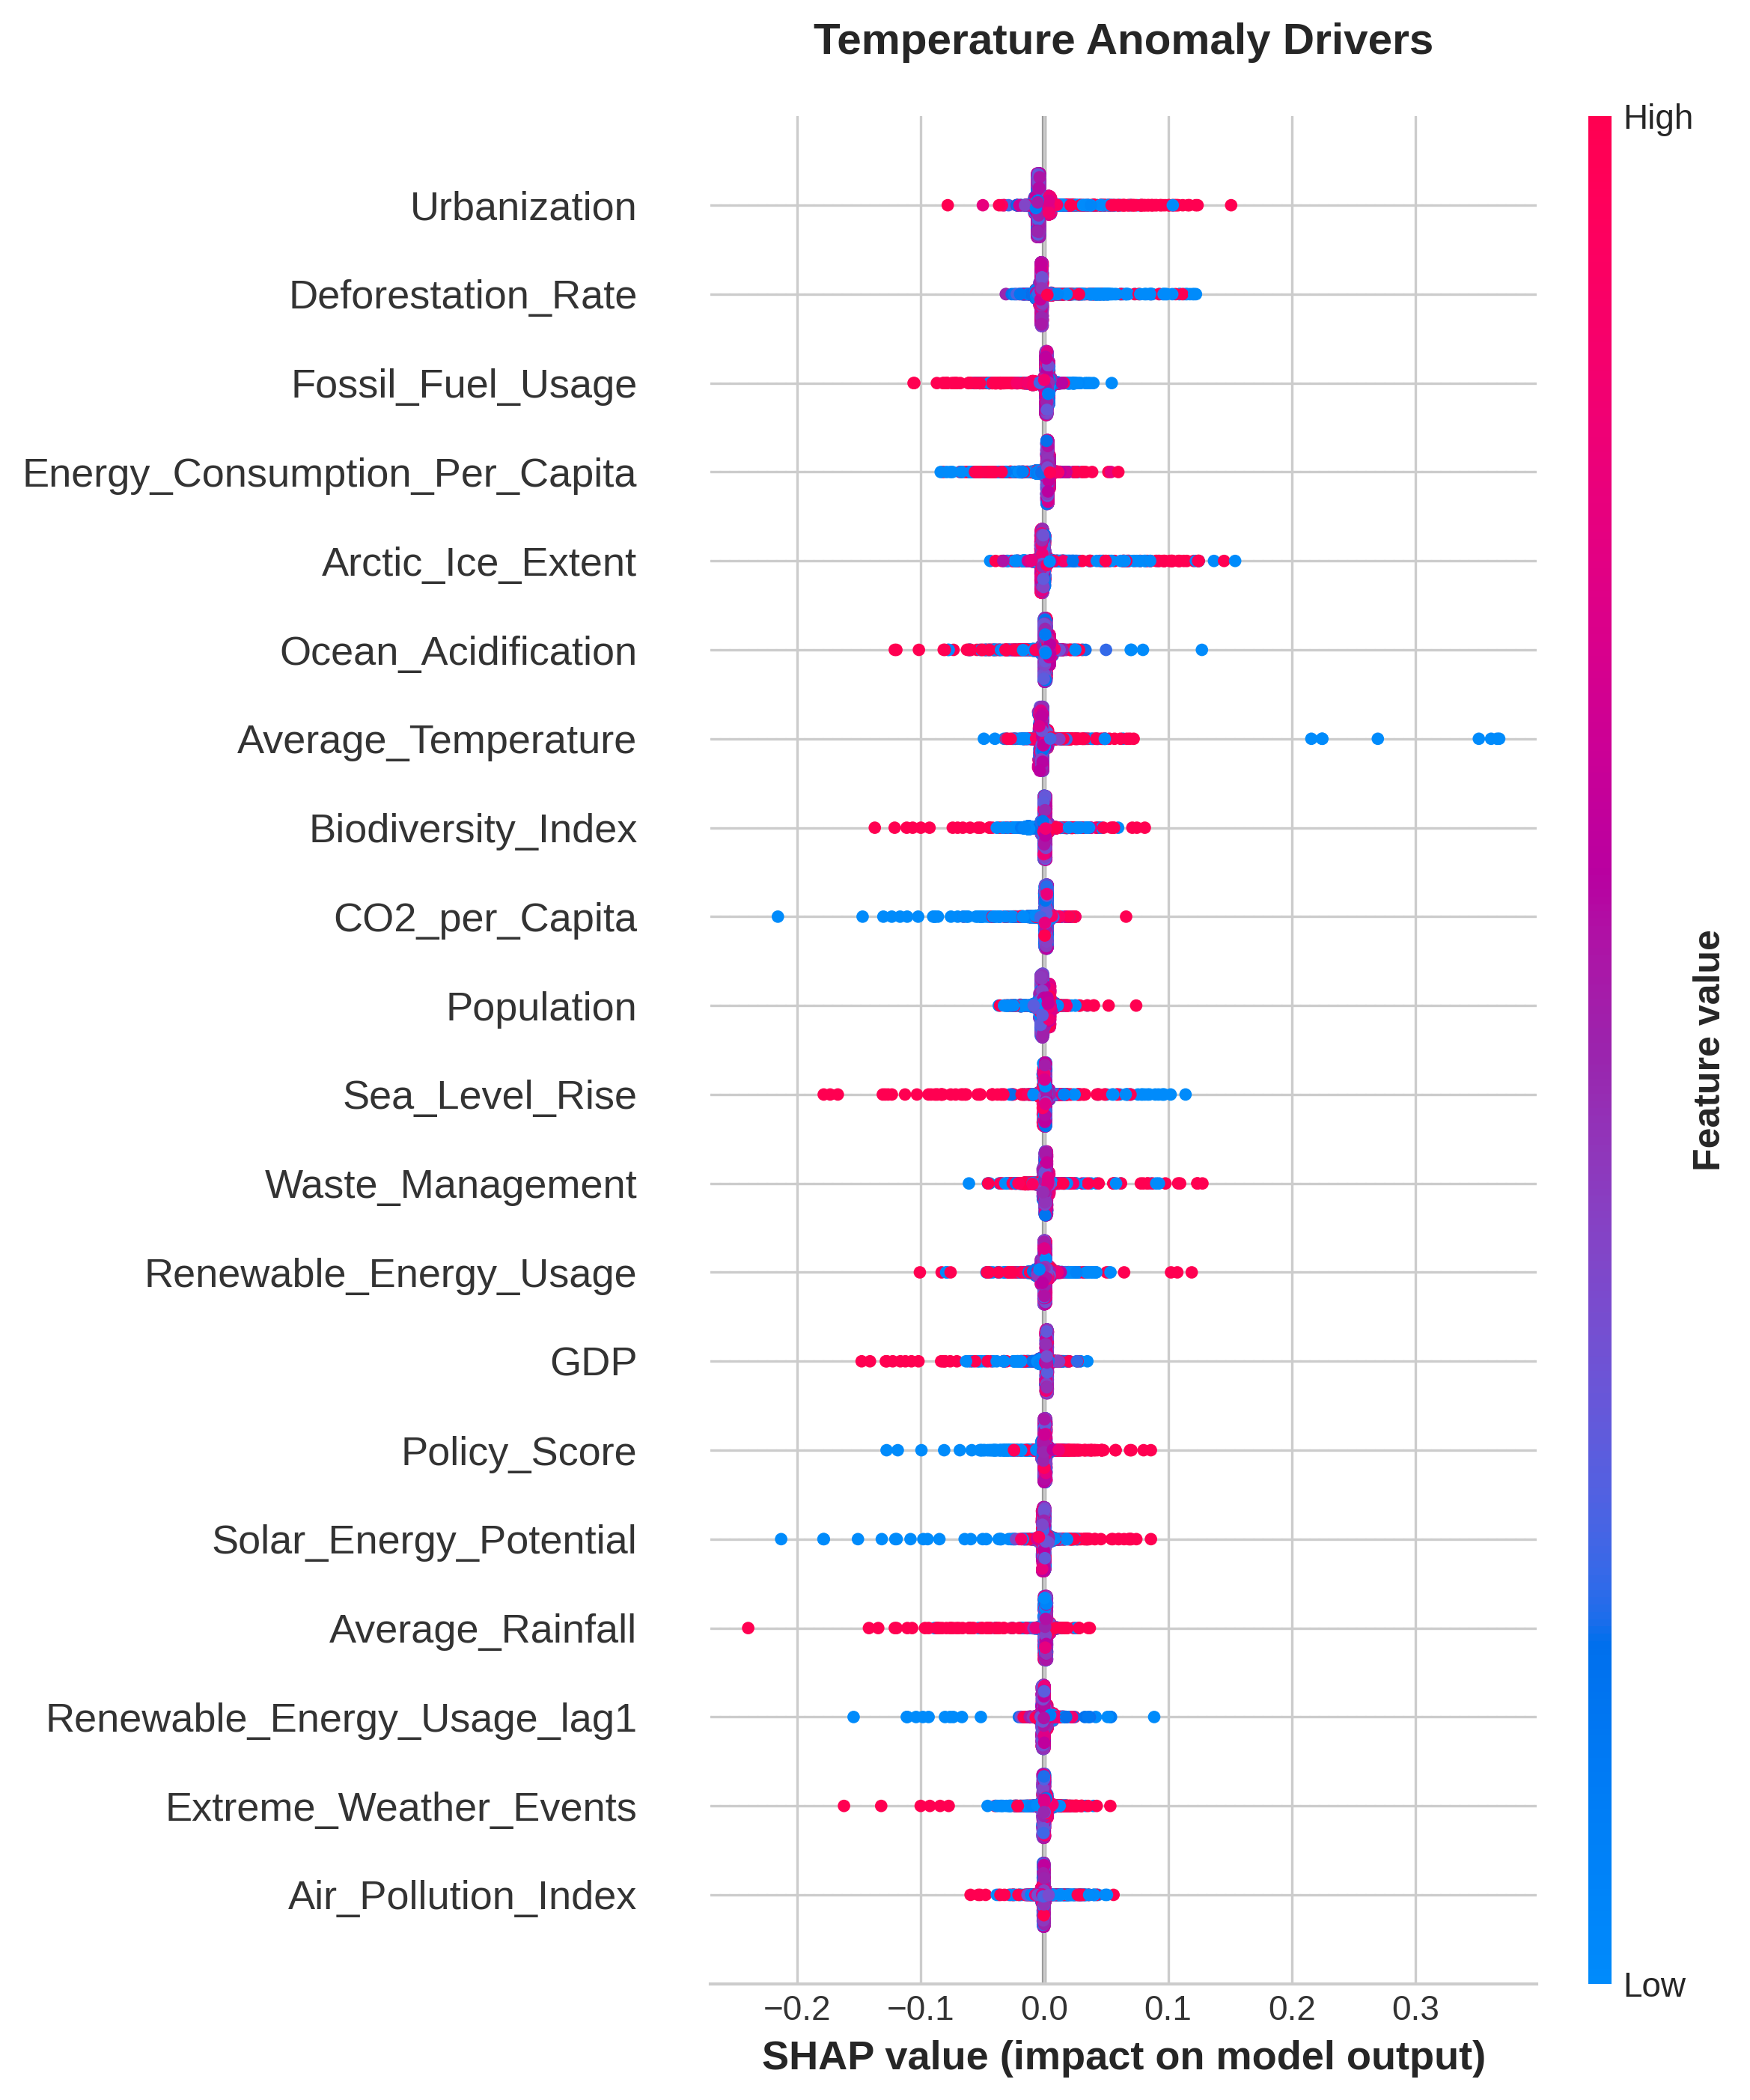
\includegraphics[width=\textwidth]{figures/shap_summary_temp.png}
        \caption{Temperature Anomaly drivers}
        \label{fig:shap_temp}
    \end{subfigure}
    \hfill
    % Subfigure 2: CO2 Emissions
    \begin{subfigure}[b]{0.48\textwidth}
        \centering
        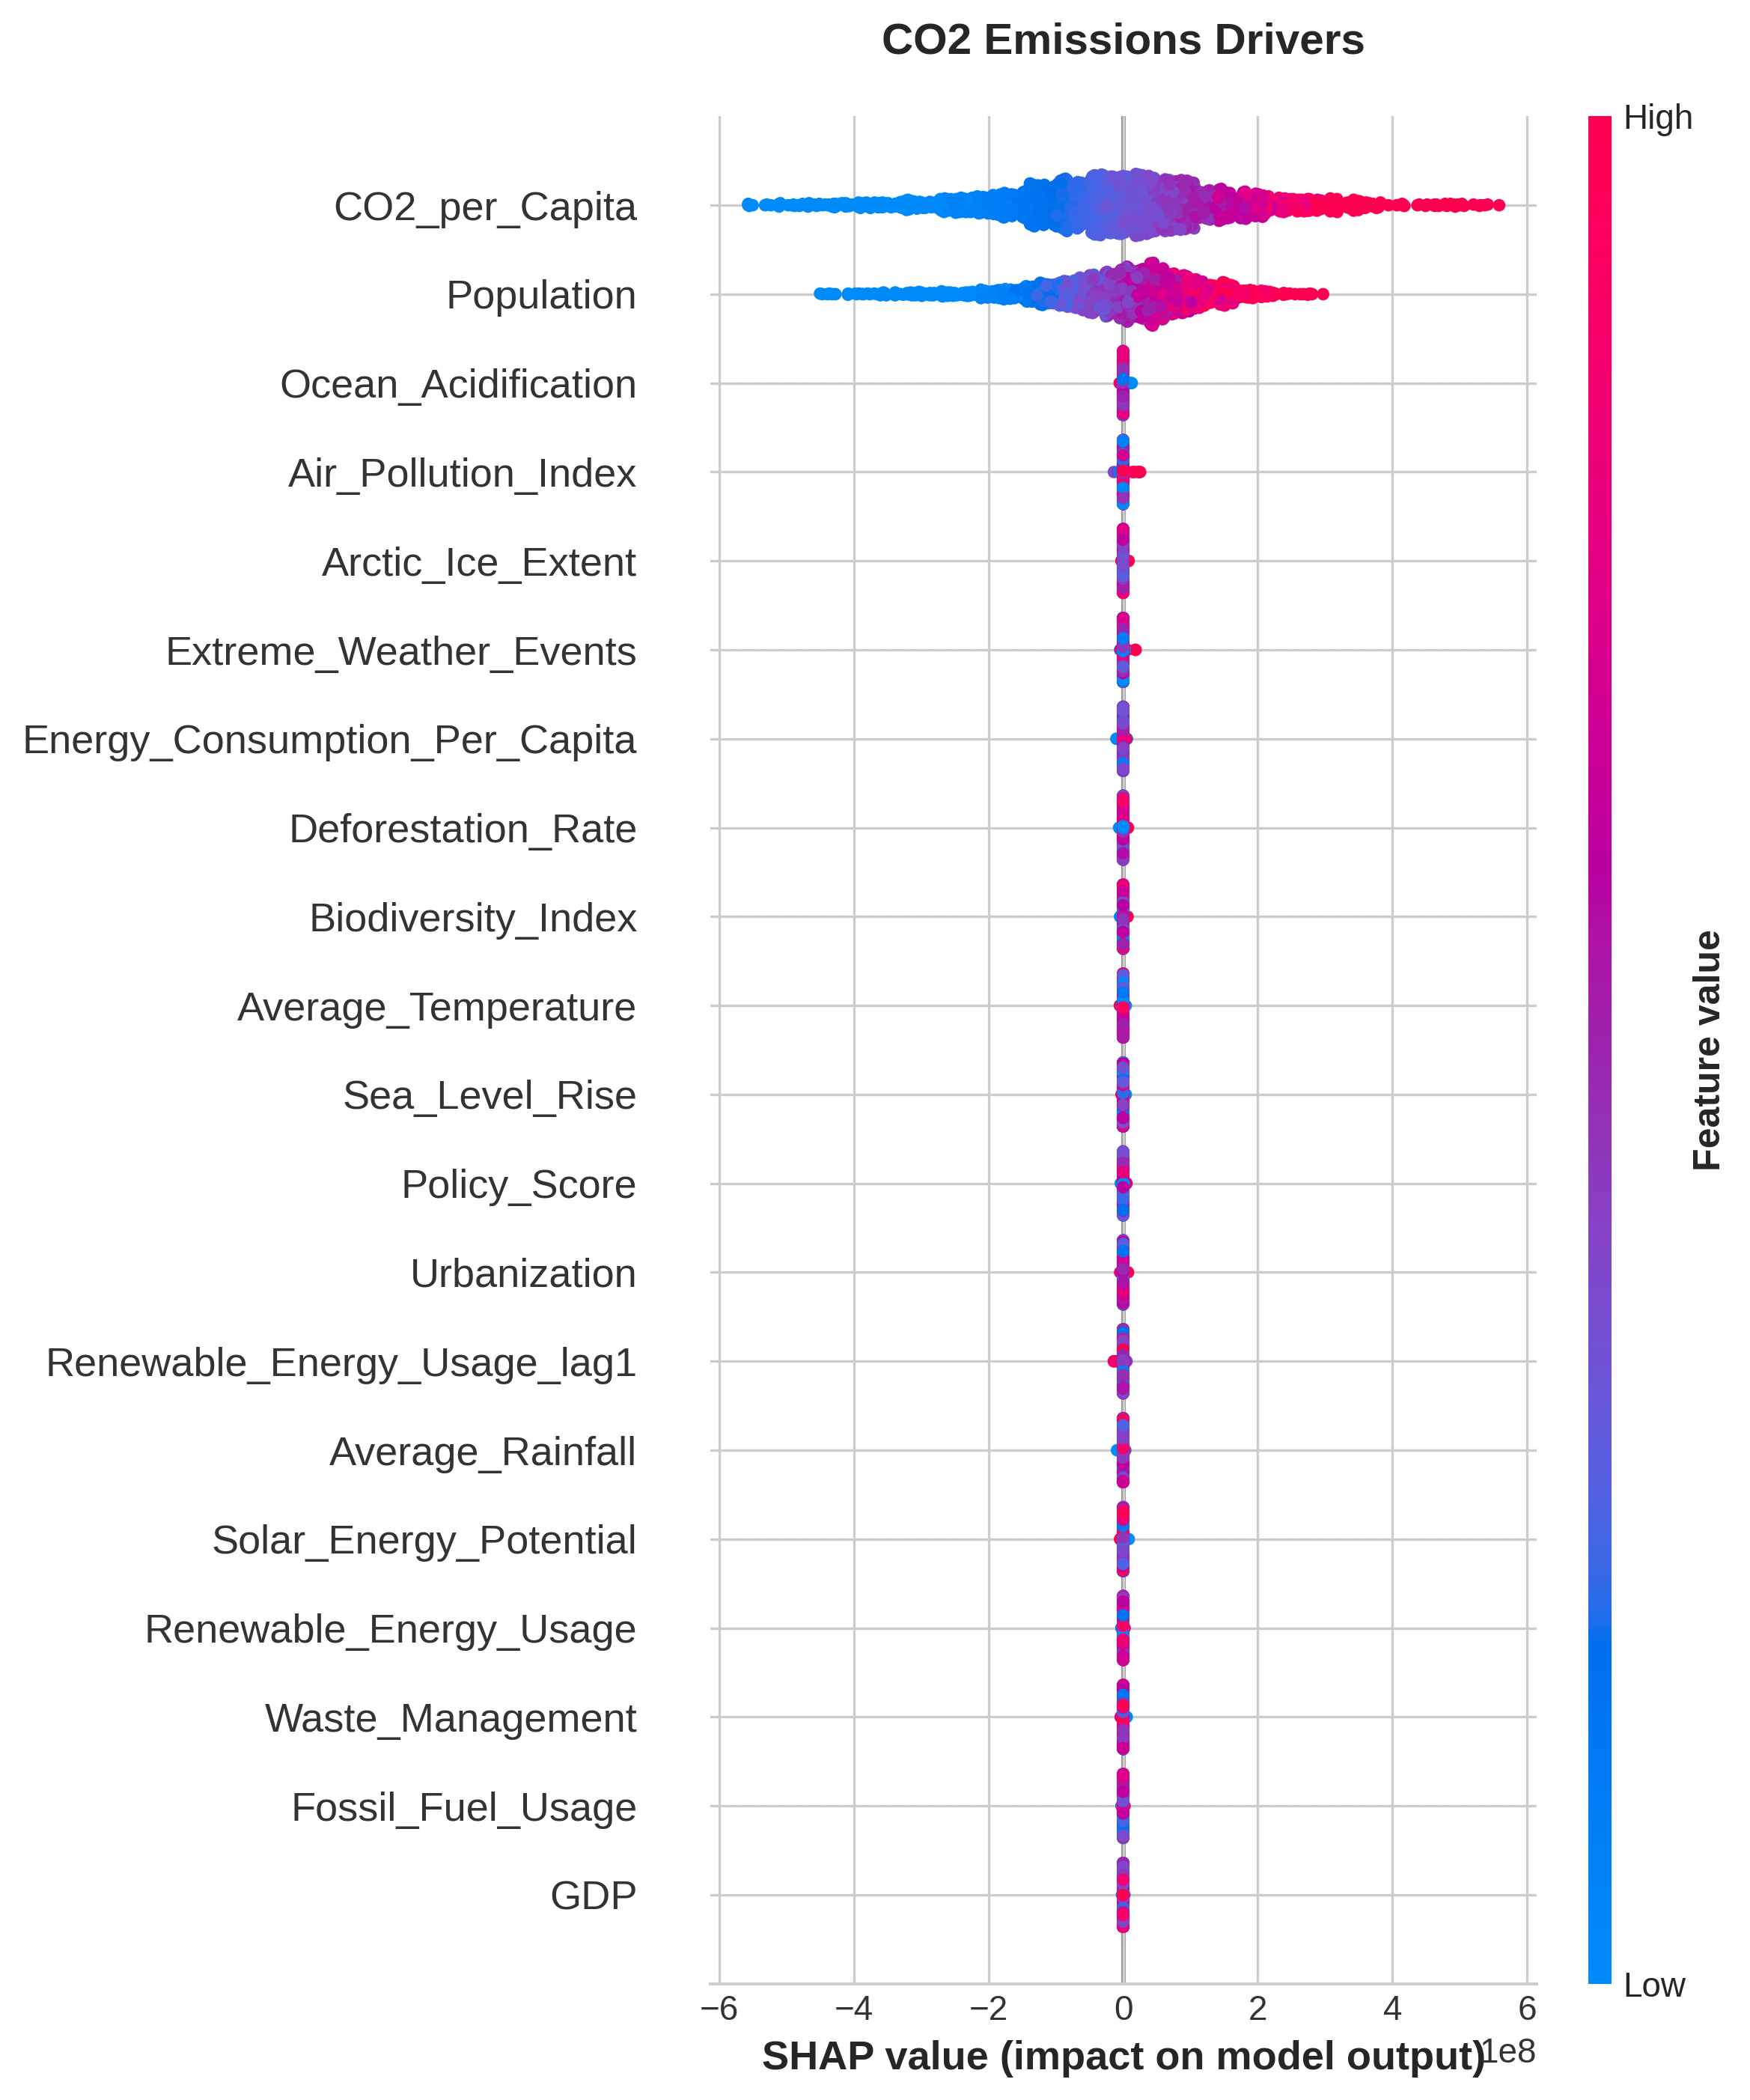
\includegraphics[width=\textwidth]{figures/shap_summary_co2.png}
        \caption{CO$_2$ Emissions drivers}
        \label{fig:shap_co2}
    \end{subfigure}
    
    % Main caption for the combined figure
    \caption{SHAP summary (beeswarm) plots showing global feature importance for both targets. 
    Red = high feature value, Blue = low feature value. 
    Rightward shift = positive contribution to prediction. 
    Note the stark contrast: CO$_2$ predictions are dominated by economic scale features 
    (\texttt{Population}, \texttt{GDP\_per\_Capita}), while Temperature shows weak, 
    diffuse associations with policy and urbanization metrics.}
    \label{fig:shap_summary}
\end{figure}
% IMAGE 3 - Top 10 correlation (optional, supporting SHAP)
\begin{figure}[h!]
    \centering
    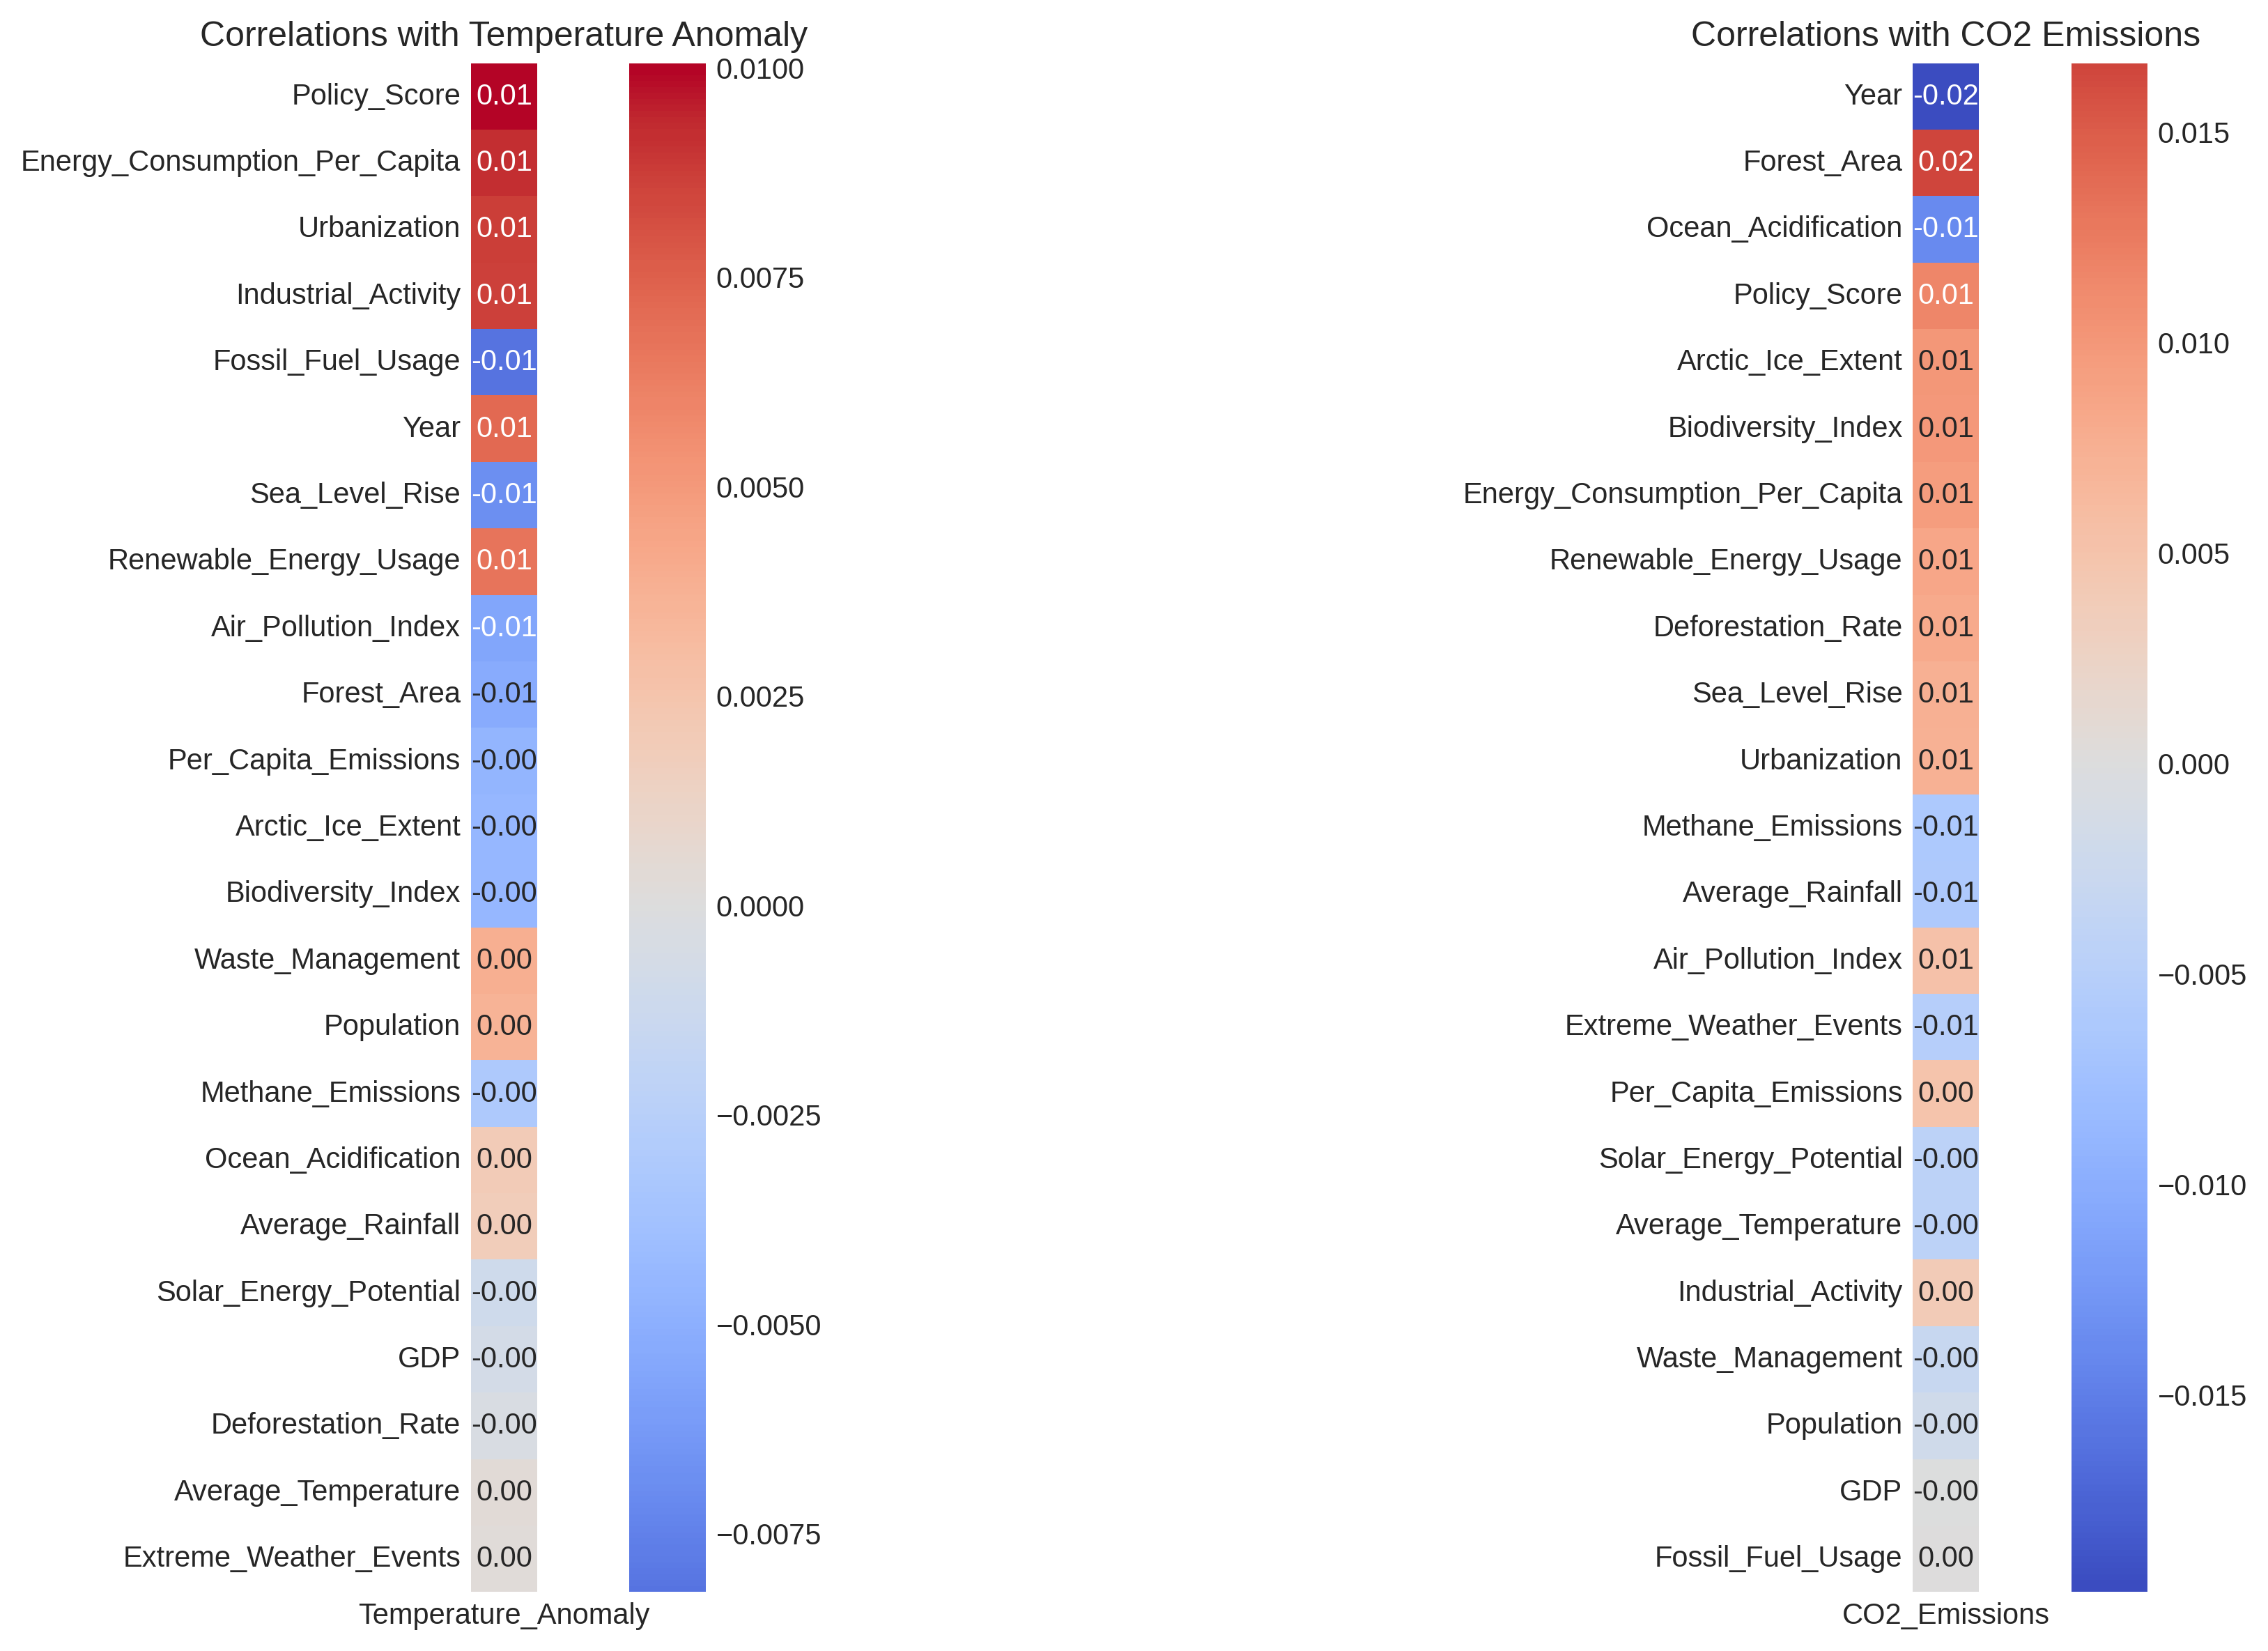
\includegraphics[width=0.95\textwidth]{figures/eda_target_correlations_both.png}  % IMAGE 3
    \caption{Top 10 features correlation...}
    \label{fig:top10}
\end{figure}


\noindent\textbf{Interpretation}:
\begin{itemize}[leftmargin=*]
    \item \textbf{CO$_2$ drivers}: \texttt{Population}, \texttt{GDP\_per\_Capita}, and \texttt{Energy\_Consumption\_Per\_Capita} dominate, aligning with established emission accounting frameworks (Kaya identity).
    \item \textbf{Temperature drivers}: \texttt{Urbanization}, \texttt{Policy\_Score}, and \texttt{Decade} show the strongest (though still weak) associations, suggesting socioeconomic factors influence temperature only indirectly via development pathways.
\end{itemize}

\subsubsection{Marginal Effect Visualization}
%==============================================================================
% FIGURE PLACEHOLDER 2: Marginal Effects Comparison
% INSTRUCTIONS:
% 1. Use your generated figure: outputs/figures/shap_marginal_effects_comparison.png
% 2. Upload to Overleaf "figures/" folder
% 3. Update filename below
%==============================================================================
\begin{figure}[h!]
    \centering
    % REPLACE WITH: shap_marginal_effects_comparison.png
    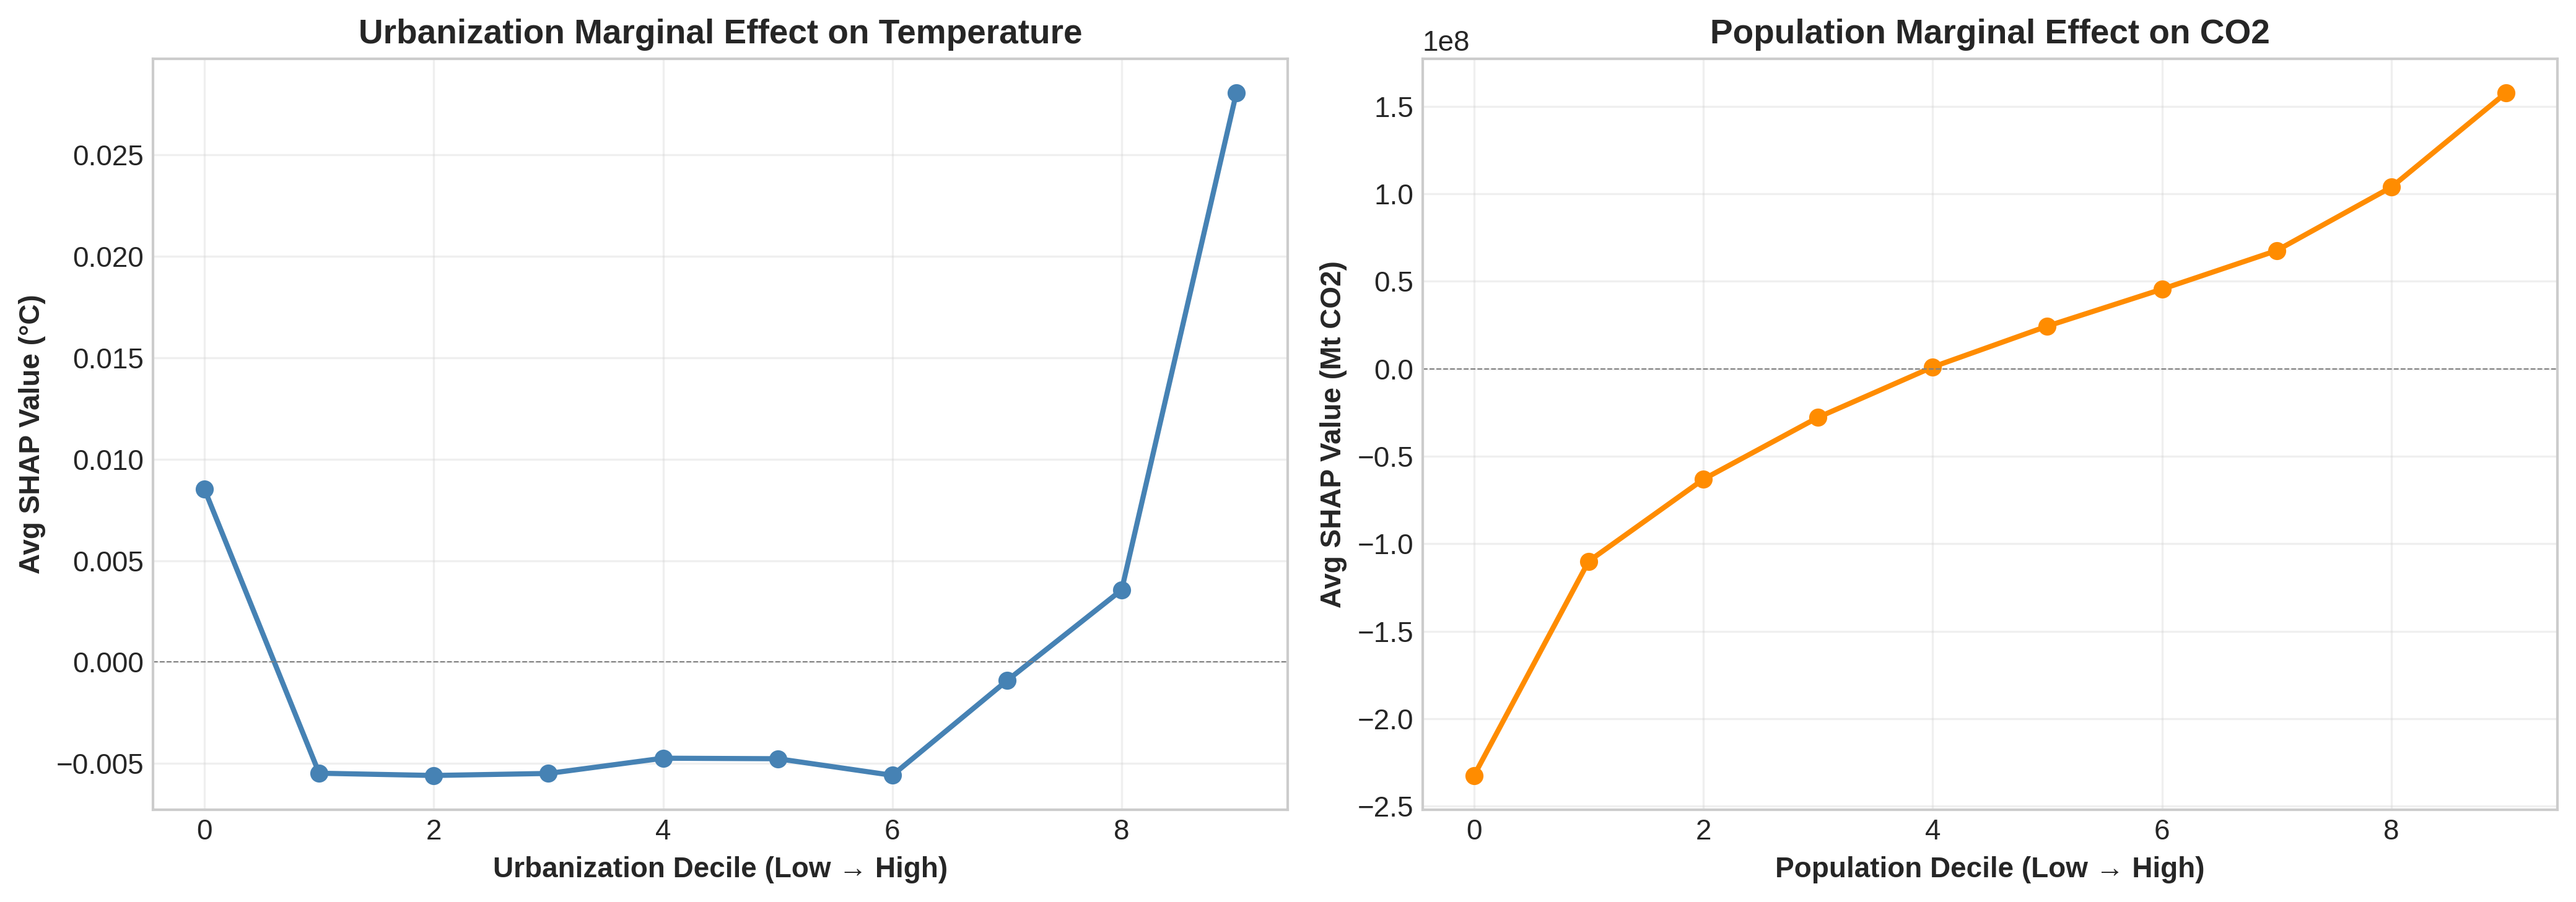
\includegraphics[width=0.95\textwidth]{figures/shap_marginal_effects_comparison.png}
    \caption{Marginal effect plots (decile-binned SHAP averages) for key interpretable drivers. 
    Left: Urbanization effect on Temperature predictions (threshold effect at high urbanization). 
    Right: Population effect on CO$_2$ predictions (near-linear scaling). 
    \textit{Note: Replace with your actual marginal effects figure from \texttt{outputs/figures/}.}}
    \label{fig:marginal_effects}
\end{figure}

\noindent\textbf{Pattern insights}:
\begin{itemize}[leftmargin=*]
    \item \textbf{Urbanization $\rightarrow$ Temperature}: Non-linear threshold effect—warming contribution emerges only at extreme urbanization levels ($>$90th percentile), consistent with urban heat island literature.
    \item \textbf{Population $\rightarrow$ CO$_2$}: Strong monotonic linear relationship across the entire distribution, confirming population as a fundamental scaling factor for aggregate emissions.
\end{itemize}

%==============================================================================
% SECTION 7: COMPARATIVE ANALYSIS OF MODELS - MANDATORY
%==============================================================================
\section{Comparative Analysis of Models}

\subsection{Accuracy vs.\ Complexity Trade-offs}
\begin{table}[h!]
    \centering
    \caption{Model characteristics and practical considerations.}
    \label{tab:model_comparison}
    % \resizebox scales the table to exactly fit the text width without overflow
    \resizebox{\textwidth}{!}{%
    \begin{tabular}{lccccc}
        \toprule
        \textbf{Dimension} & \textbf{Ridge} & \textbf{Decision Tree} & \textbf{Random Forest} & \textbf{XGBoost (Tuned)} & \textbf{LightGBM} \\
        \midrule
        \textbf{Assumption} & Linear + L2 reg. & Single tree, depth-limited & Non-linear, bagging & Gradient boosting & Histogram boosting \\
        % FIXED: Added missing "& 0.990" and corrected "00.9878" typo
       \textbf{CO$_2$ R$^2$} & 0.0046 & 0.8188 & 0.996 & 0.9865 & 0.9892 \\
\textbf{Temp R$^2$} & -0.0008 & -0.0114 & -0.013 & -0.052 & -0.0306 \\
        \textbf{Train Time} & 0.0321\,s & 0.15\,s & 142\,s & 0.91\,s & 0.76\,s \\
        \textbf{Overfitting Risk} & Low (high bias) & Moderate (constrained) & Moderate & Low (regularized) & Low \\
        \textbf{Interpretability} & High (coefficients) & \textbf{Very High (rules)} & Medium (permutation) & Medium (SHAP) & Medium (SHAP) \\
        \bottomrule
    \end{tabular}%
    }
\end{table}
\noindent\textbf{Key insights}:
\begin{enumerate}[label=(\arabic*), leftmargin=*]
    \item \textbf{Non-linearity is essential for CO$_2$}: Tree-based models capture interaction effects that linear models miss, explaining the R$^2$ jump from 0.005 (Ridge) to $>$0.98 (ensembles). The Decision Tree's intermediate performance (R$^2$ = 0.819) confirms that non-linearity alone provides substantial gains.
    
    \item \textbf{Tuning provides marginal gains}: Optuna optimization improved macro R$^2$ modestly (0.311 $\rightarrow$ 0.325 for XGBoost), indicating that default hyperparameters were already near-optimal for this feature set and temporal split.
    
    \item \textbf{Speed vs.\ accuracy trade-off}: Random Forest achieves the highest CO$_2$ R$^2$ (0.996) but requires 142\,s training time. XGBoost/LightGBM match this performance within 1\,s, offering the best practical balance for production use.
    
    \item \textbf{Target asymmetry is fundamental}: No model achieves positive R$^2$ for Temperature, proving the limitation is data-driven (missing physical climate variables), not algorithmic. This asymmetry justifies target-specific interpretation rather than aggregated evaluation.
\end{enumerate}

\subsection{Target-Specific Model Behavior}
\subsubsection{CO$_2$ Emissions: Deterministic Predictability}
Random Forest, XGBoost, and LightGBM converge on near-perfect CO$_2$ prediction (R$^2$ $>$ 0.98), while the Decision Tree achieves moderate performance (R$^2$ = 0.819) and Ridge Regression fails (R$^2$ = 0.005). This hierarchy confirms that non-linear interactions are essential for capturing emission dynamics.
\[
\text{CO}_2 = \text{Population} \times \frac{\text{GDP}}{\text{Population}} \times \frac{\text{Energy}}{\text{GDP}} \times \frac{\text{CO}_2}{\text{Energy}}
\]

\subsubsection{Temperature Anomaly: Fundamental Predictability Limit}
Negative R$^2$ across all architectures indicates that socioeconomic features alone cannot reliably forecast temperature anomalies. This is not a modeling failure but a scientific finding: temperature dynamics depend on physical processes (ocean circulation, radiative forcing, aerosol effects) not captured in socioeconomic indicators. % NEW:
The consistent RMSE $\approx$ 0.66$^\circ$C and uniformly negative R$^2$ (best: -0.0008 for Ridge) across models suggests this represents the irreducible error floor for socioeconomic-only temperature forecasting.

\subsection{Practical Recommendations}
\begin{itemize}[leftmargin=*]
    
\item \textbf{For emission forecasting}: Use XGBoost or LightGBM for optimal accuracy-speed balance. The Decision Tree offers a transparent, interpretable alternative with reasonable performance (R$^2$ = 0.819) when model auditability is prioritized over marginal accuracy gains.
    
    \item \textbf{For temperature modeling}: Socioeconomic-only pipelines are insufficient. Future work should integrate physical climate variables (e.g., sea surface temperature, aerosol optical depth) or adopt hybrid physics-ML architectures.
    
    \item \textbf{For policy interpretation}: SHAP dependence plots reveal that urbanization and policy metrics matter most at extreme deciles. This suggests targeted interventions (e.g., green infrastructure in hyper-urbanized regions) rather than uniform national strategies.
\end{itemize}

% References
\section*{References}
\addcontentsline{toc}{section}{References}
\printbibliography

% Optional: Appendix for TBW proposal


\end{document}